\documentclass[tikz,border=10pt]{standalone}
\usepackage[T1]{fontenc}
\usepackage{helvet}
\renewcommand{\familydefault}{\sfdefault}
\usepackage{tikz}
\usetikzlibrary{arrows.meta,positioning,shapes.multipart,shapes.geometric,fit,backgrounds,calc,shadows}

\definecolor{navy}{HTML}{1F3A5F}
\definecolor{teal}{HTML}{0C6B58}
\definecolor{amber}{HTML}{D9822B}
\definecolor{crimson}{HTML}{B42318}
\definecolor{violet}{HTML}{6B21A8}
\definecolor{sky}{HTML}{2186EB}
\definecolor{slate}{HTML}{486581}
\definecolor{mist}{HTML}{F0F4F8}
\definecolor{line}{HTML}{9FB3C8}

\tikzset{
  >={Stealth[length=2.6mm]},
  box/.style={draw=navy, very thick, rounded corners=3pt, fill=white, align=center,
    inner sep=5pt, font=\small, minimum height=9mm},
  softbox/.style={box, draw=slate, thick, fill=mist},
  layer/.style={draw=line, dashed, rounded corners=6pt, inner sep=7pt},
  layertitle/.style={font=\bfseries\small, text=slate, anchor=north west},
  flow/.style={->, thick, draw=navy},
  dflow/.style={->, thick, draw=slate, dashed},
  lbl/.style={font=\scriptsize, text=slate, fill=white, inner sep=1.5pt},
  umlclass/.style={draw=navy, thick, fill=white, rectangle split, rectangle split parts=3,
    rectangle split part fill={navy!12,white,white}, align=left, font=\scriptsize,
    inner sep=3pt, text width=#1},
  umlclass/.default=38mm,
}

\tikzset{
  actor/.style={box, minimum width=2.5cm, minimum height=1.1cm, font=\small\bfseries},
  life/.style={draw=line, thick, dashed},
  call/.style={->, thick, draw=navy},
  reply/.style={->, thick, dashed, draw=slate},
  msg/.style={font=\scriptsize, fill=white, inner sep=1.5pt},
}
\begin{document}
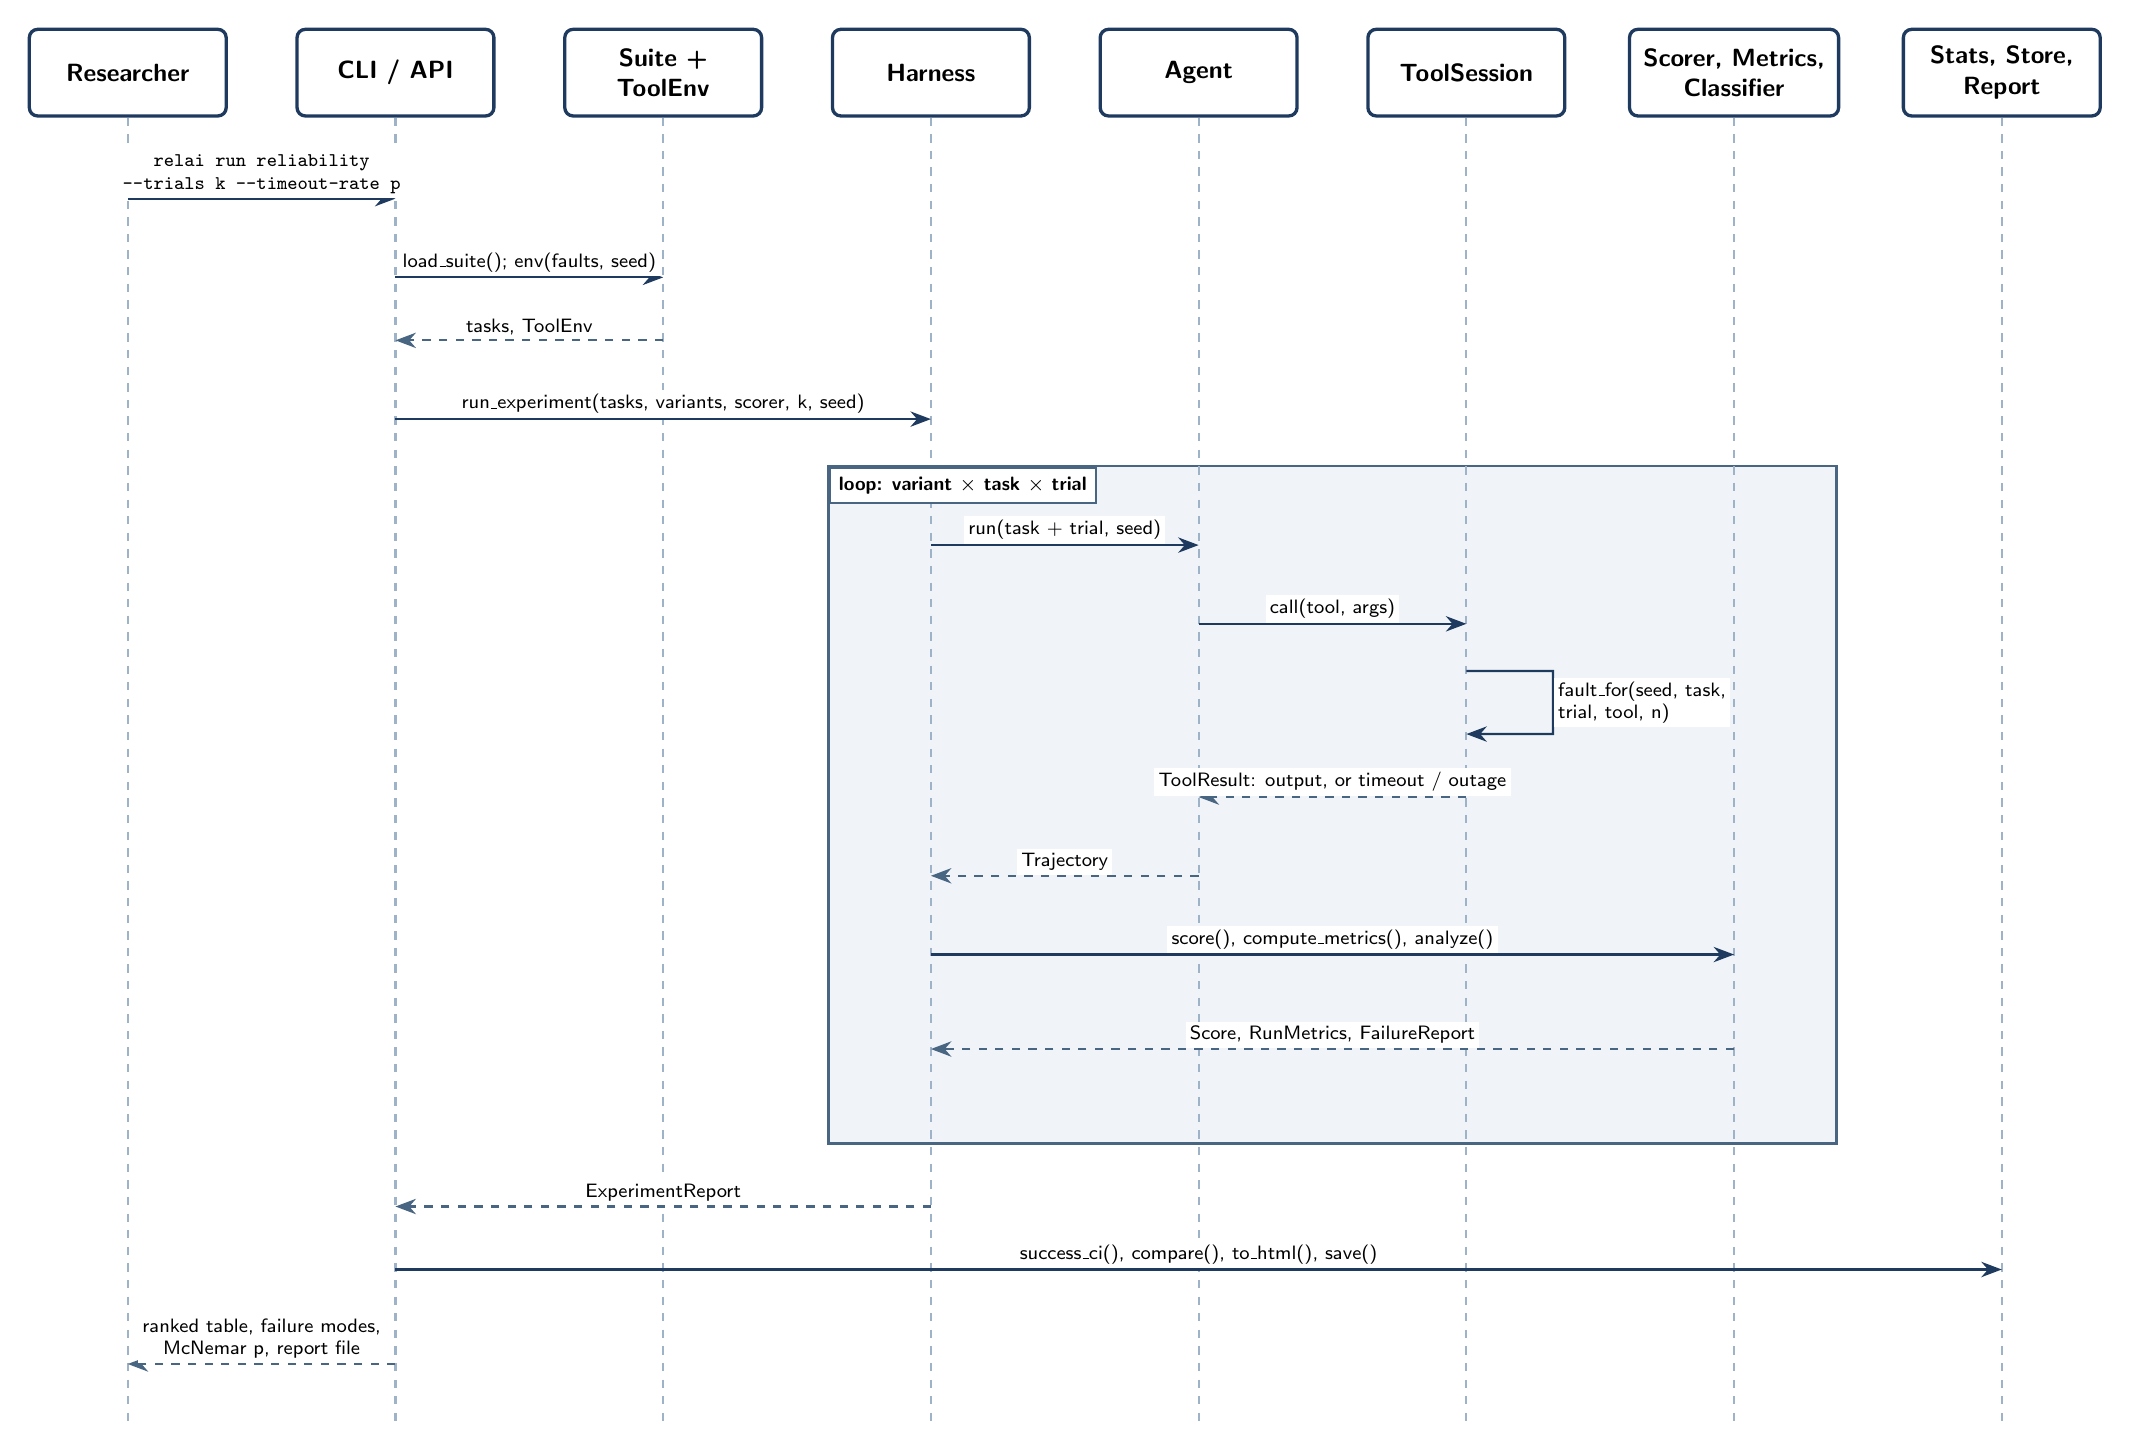
\begin{tikzpicture}[x=1cm,y=1cm]
  \def\bottom{-17.2}
  \foreach \name/\x/\label in {user/0/Researcher, cli/3.4/{CLI / API}, suite/6.8/{Suite +\\ToolEnv}, harness/10.2/Harness, agent/13.6/Agent, session/17.0/ToolSession, analysis/20.4/{Scorer, Metrics,\\Classifier}, out/23.8/{Stats, Store,\\Report}} {
    \node[actor] (\name) at (\x,0) {\label};
    \draw[life] (\name.south) -- (\x,\bottom);
  }
  \newcommand{\call}[4]{\draw[call] (#1,#3) -- node[msg, above] {#4} (#2,#3);}
  \newcommand{\reply}[4]{\draw[reply] (#1,#3) -- node[msg, above] {#4} (#2,#3);}

  \draw[call] (0,-1.6) -- node[msg, above, align=center] {\texttt{relai run reliability}\\\texttt{-{}-trials k -{}-timeout-rate p}} (3.4,-1.6);
  \call{3.4}{6.8}{-2.6}{load\_suite(); env(faults, seed)}
  \reply{6.8}{3.4}{-3.4}{tasks, ToolEnv}
  \call{3.4}{10.2}{-4.4}{run\_experiment(tasks, variants, scorer, k, seed)}

  \begin{scope}[on background layer]
    \fill[mist] (8.9,-5.0) rectangle (21.7,-13.6);
    \draw[slate, thick] (8.9,-5.0) rectangle (21.7,-13.6);
  \end{scope}
  \node[draw=slate, thick, fill=white, font=\scriptsize\bfseries, anchor=north west] at (8.9,-5.0) {loop: variant $\times$ task $\times$ trial};

  \call{10.2}{13.6}{-6.0}{run(task + trial, seed)}
  \call{13.6}{17.0}{-7.0}{call(tool, args)}
  \draw[call] (17.0,-7.6) -- ++(1.1,0) -- node[msg, right, align=left] {fault\_for(seed, task,\\trial, tool, n)} ++(0,-0.8) -- (17.0,-8.4);
  \reply{17.0}{13.6}{-9.2}{ToolResult: output, or timeout / outage}
  \reply{13.6}{10.2}{-10.2}{Trajectory}
  \call{10.2}{20.4}{-11.2}{score(), compute\_metrics(), analyze()}
  \reply{20.4}{10.2}{-12.4}{Score, RunMetrics, FailureReport}

  \reply{10.2}{3.4}{-14.4}{ExperimentReport}
  \call{3.4}{23.8}{-15.2}{success\_ci(), compare(), to\_html(), save()}
  \draw[reply] (3.4,-16.4) -- node[msg, above, align=center] {ranked table, failure modes,\\McNemar p, report file} (0,-16.4);
\end{tikzpicture}
\end{document}
